%----------------------------------------------------------------------------------------
%	PACKAGES AND THEMES
%----------------------------------------------------------------------------------------
\documentclass[aspectratio=169,xcolor=dvipsnames,handout]{beamer}
\usetheme{Darmstadt}
\usecolortheme{seahorse}

\usepackage[hangul]{kotex}

\usepackage{hyperref}
\usepackage{amsfonts, amssymb}
\usepackage{graphicx} % Allows including images
\usepackage{array, booktabs, multicol, multirow} % Allows the use of \toprule, \midrule and \bottomrule in tables
\setbeamercovered{transparent}

\newcommand{\R}{\mathbb{R}}
\newcommand{\y}{\mathbf{y}}

%----------------------------------------------------------------------------------------
%	TITLE PAGE
%----------------------------------------------------------------------------------------

\title[우파적 자유주의]{우파적 자유주의} % The short title appears at the bottom of every slide, the full title is only on the title page
\subtitle{경제정의와 불평등}

\author[오성재]{오성재}

\institute[HNU] % Your institution as it will appear on the bottom of every slide, may be shorthand to save space
{
    한남대학교 \\
    탈메이지 교양학부 \\
}
\date{\today} % Date, can be changed to a custom date


%----------------------------------------------------------------------------------------
%	PRESENTATION SLIDES
%----------------------------------------------------------------------------------------

\begin{document}

\begin{frame}
    \titlepage
\end{frame}

\begin{frame}{목차}
    \tableofcontents
\end{frame}

\section{들어가늘 말}

\begin{frame}[<+->]
\frametitle{화폐}
    \begin{itemize}
        \item 화폐의 역할 : 
        \begin{itemize}
            \item 교환수단.
            \item 가치척도.
            \item 가치저장.
        \end{itemize}
        \item 가치의 종류 : 
        \begin{itemize}
            \item 교환가치.
            \item 사용가치.
        \end{itemize}
        
    \end{itemize}
\end{frame}

\begin{frame}[<+->]
\frametitle{우파적 자유주의}
    \begin{itemize}
        \item 우파적 자유주의(고전적 자유주의)는 자유(liberty)와 효용(utility)의 결합.
    \end{itemize}
\end{frame}

\section{우파적 자유주의}
\begin{frame}[<+->]
\frametitle{하이에크}
    \begin{columns}
        \begin{column}{.5\textwidth}
            \begin{figure}
                \centering
                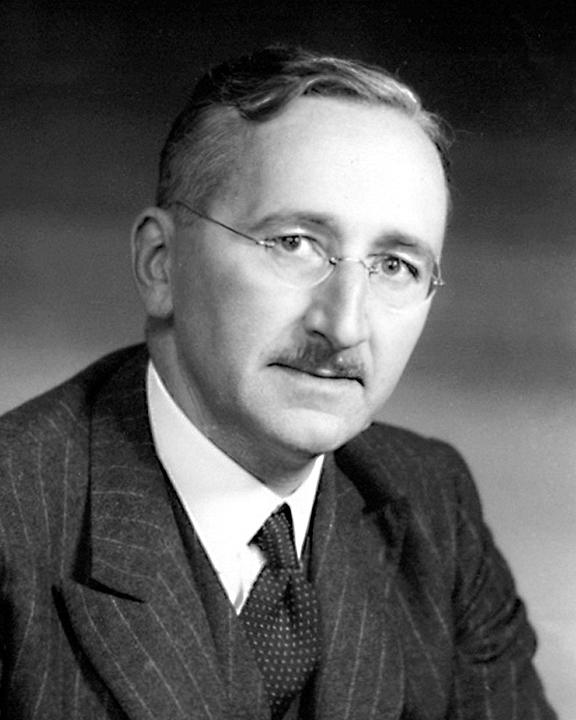
\includegraphics[width=.5\textwidth]{pic/Hayek_portrait.jpg}
            \end{figure}
        \end{column}    
        \begin{column}{.5\textwidth}
            \begin{itemize}
            \item Friedrich Hayek(1898-1992)
            \item 오스트리아 출생, 영국국적.
            \item 1974년 노벨 경제학상 수상.
            \item 경제학, 철학, 법학
            \end{itemize}
        \end{column}    
    \end{columns}
\end{frame}

\begin{frame}[<+->]
\frametitle{결과주의 분류}
    \begin{itemize}
        \item 추구하는 가치에 따른 분류:
        \begin{itemize}
            \item 쾌락주의 : 즐거움과 고통이 없는 상태만을 추구해야 한다.
            \item 선호주의 : 선호의 만족이 좋은 것이고 불만족은 나쁜 것이다.
            \item 완전주의 : 훌륭한 인간적 삶(?)을 달성하는 것이 중요하다.
        \end{itemize}
    \end{itemize}
\end{frame}

\begin{frame}[<+->]
\frametitle{하이에크의 결과주의}
    \begin{itemize}
        \item 정의로운 행위에 따른 분류 :
        \begin{itemize}
            \item 직접적 결과주의 : 행위는 그것이 가장 바람직한 결과를 초래하는 한 도덕적으로 옳다.
            \item 간접적 결과주의 : 어떤 \textbf{규칙}을 준수하는 것이 대체로 가장 바람직한 결과를 가져올 때, 그 규칙에 부합하는 행위가 옳다.
        \end{itemize}
        \item 하이에크 : 선호와 개인의 자유에 관한 간접적 결과주의.
    \end{itemize}
\end{frame}

\begin{frame}[<+->]
\frametitle{우파적 자유주의}
    \begin{itemize}
        \item 하이에크의 결과주의는 충분주의를 반영하는 곱(product)의 결과주의.
        \begin{exampleblock}{다양한 사회지표(social index)}
            총합, 평균, 편차, 최소, 곱.
        \end{exampleblock}
    \end{itemize}
    \begin{center}
    \begin{table}
    \begin{tabular}{lccc}
        \toprule
        & \text { 빈층 } & \text { 중산층 } & \text { 부유층 } \\
        \hline \text { 충분주의 } & 1 & 4 & 18 \\
        \text { 강건한 중산층 } & 2 & 6 & 14 \\
        \text { 극단적 불평등 } & 0.6 & 3 & 30 \\
        \text { 충분주의 및 극단적 불평등 } & 1 & 3 & 29 \\
        \bottomrule
    \end{tabular}
    \caption{다양한 소득분포}
    \end{table}
    \end{center}
\end{frame}

\section{자유로운 시장과 법치주의}
\begin{frame}[<+->]
\frametitle{자생적 질서와 카탈락시(Catallaxy)}
\begin{itemize}
    \item 사회적 목표(선호와 개인의 자유)는 자유 시민들의 창의력을 통해서 가장 잘 달성.
    \item 이러한 주장은 역사적 사실로 뒷받침.
    \begin{exampleblock}{인류사의 주요경제체제}
    \begin{itemize}
        \item 수렵사회 : 자연물을 단순히 채취함.
        \item 농경사회 : 인력에 의한 생산활동 시작.
        \item 중상주의 : 금=경제력.
        \item 자본주의 : 생산=경제력.
        \item 공산주의 : 사적 소유권 철폐.
    \end{itemize}
    \end{exampleblock}
\end{itemize}
\end{frame}

\begin{frame}[<+->]
\frametitle{자유시장경제}
    \begin{itemize}
    \item 공산주의와 (시장)자본주의 간에 진영대립에서 시장의 우월성을 입증.
    \begin{itemize}
        \item  공산주의 : 중앙집권적 계획경제.
        \item  자본주의 : 가격기구, 수요와 공급의 법칙 등등.
    \end{itemize}
        \item 사익(self-interest)추구만을 강조하더라도 사회적 목표가 달성 가능.
        \item 시장경제는 인간의 제한된 지식에 근거할 때, 생산과 분배에서 가장 효율적인 제체.
        \item 시장경제는 경제생활에서 개인의 자유를 보장.
    \end{itemize}
\end{frame}

\begin{frame}[<+->]
\frametitle{자유(Liberty)}
    \begin{itemize}
        \item 자유의 중요성. 
        \begin{itemize}
            \item 자유는 그 자체로 좋은 것.
            \item 번영의 수단.
        \end{itemize}
        \item 자유의 정의 : 
        \begin{itemize}
            \item  자유는 타인에 의한 강압이 없는 상태.
            \item  강압은 개인의 행동이 타인의 목적을 위해 타인의 의지에 따를 때 발생.
        \end{itemize}
    \end{itemize}
\end{frame}

\begin{frame}[<+->]
\frametitle{법치주의(Rule of Law)}
    \begin{itemize}
        \item 법은 구성원의 자유, 평화, 안전, 번영을 위해 필요.
        \item 법치주의의 요건을 충족하는 법만이 그 법을 따르는 구성원들의 자유와 양립.
        \item 법과 명령은 원천, 대상, 방법 세 가지에서 구분.
        \begin{itemize}
            \item 법은 적절한 입법기관에 의해 제정.
            \item 법은 특정한 사인이 아닌 전체 구성원을 동등하게 구속(bind)함.
            \item 법은 특정인에게 특정 행동을 지시하지 않음; 단순히 행위자의 결정에 고려해야 할 추가 정보를 제공.
        \end{itemize}
    \end{itemize}
\end{frame}

\begin{frame}[<+->]
\frametitle{법치주의(Rule of Law)}
    \begin{itemize}
        \item 법은 법치주의을 실현을 위해 다음과 같은 특성을 지녀야 함.
        \begin{itemize}
            \item 추상적(abstract)이고 일반적(general)이어야.
            \item 공개적으로 공표되고 공포되어야. 
            \item 모두에게 동등하게 적용되어야.
        \end{itemize}
        \item 법치주의을 실현을 위해 헌법은 다음과 같은 내용을 가져야. 
        \begin{itemize}
            \item 권력분립.
            \item 법 집행에서 권한을 남용할수 없게 하는 안전장치. 
            \item 구성원에게 기본적 자유권(언론, 집회, 종교, 재산권) 보장.
        \end{itemize}
    \end{itemize}
\end{frame}

\begin{frame}[<+->]
\frametitle{정부의 (비)강제적 기능}
    \begin{itemize}
        \item 법의 지배는 자유에 있어 필요조건이지만 충분조건이 아님.
        \begin{itemize}
            \item  자유를 누리기 위해 법은 국가가 수행해야할 행위들을 규정해야.
        \end{itemize}
        \item 법의 지배는 정부의 기능 가운데 금지, 허가, 필요를 규정.
        \begin{itemize}
            \item  금지 : 법의 지배에 맞지 않는 강압적 권력을 행사.
            \item  필요 : 구성원의 안전, 재산, 계약의 권리 등등.
            \item  허가 : 공공재(예: 기간시설, 생명선, 재난구호 등) 공급 및 구휼.
        \end{itemize}
        \item 이러한 행위를 수행하기 위해 국가는 조세를 할 수 있음. 그러나 조세가 재분배 기능을 수행하는 것은 엄격히 금해야.
    \end{itemize}
\end{frame}

\section{우파적 자유주의의 분배정의}
\begin{frame}[<+->]
\frametitle{하이에크의 분배정의 원칙}
    \begin{itemize}
        \item 효용의 원칙 : 정의로운 사회(그리고 정의로운 법과 제도)는 사회의 목적(효용과 자유)을 가장 잘 촉진하는 사회.
        \item 자유의 원칙 : 정당한 자원의 분배는 자유 시장에서의 자발적인 거래의 결과인 분배.
        \item 충분주의 원칙 : 사회가 극도의 빈곤을 허용해서는 안되며 모든 사회 구성원이 최소한의 기본 소득을 보장함으로써 만족할 수 있는 최소한의 품위 있는 삶을 영위할 수 있도록 보장해야.
    \end{itemize}
\end{frame}

\begin{frame}[<+->]
\frametitle{공리vs자유}
    \begin{itemize}
        \item 가장 효율적인 법률 및 제도가 자유를 가장 잘 존중하고 보호하고 보존하는 제도인가?
        \begin{itemize}
            \item  자유와 행복의 기회 극대화.
            \item  사회구성원의 자발적인 교류가 만들어내는 비효율성.
            \item  자발적인 교류를 제한하거나 재분배를 통한 사회후생의 개선.
        \end{itemize}
        \item 하이에크와 우익 자유주의자는 실증적 전제로 두 원칙간의 갈등을 회피.
        \begin{itemize}
            \item  자유의 체제가 가장 효율적인 체제.
            \item  자발적인 교환에서 발생하는 분배가 최적의 접근 가능한 분배.
        \end{itemize}
        \item  인간의 무지에 의해 자유주의 체제를 개선하려는 모든 시도는 역효과를 일으키고 비효율을 유발.
    \end{itemize}
\end{frame}

\begin{frame}[<+->]
\frametitle{다른 분배정의 원칙에 대한 비판}
    \begin{itemize}
        \item 우선, 공로, 평등의 원칙을 적용하려는 어떤 시도도 정부의 시장에 대한 미세하고 복잡한 접근이 필요하고 따라서 법에 의한 지배를 훼손.
        \item 불평등은 개인의 자유와 각자가 자원에 접근할 수 있는 기회를 최대화하는 체제를 가지는데 대한 피할 수 없는 댓가.
        \item 하이에크는 대부분의 재회에 대한 접근 가능성에서 자유시장경제가 가난한 사람들에게도 다른 체제보다 우월하다고 주장.
        \begin{itemize}
            \item  자유시장체제에서 가난한 사람들이라 하더라도 다른 어떤 체제보다 더 나은 삶(의 기회)을 누림.
        \end{itemize}
    \end{itemize}
\end{frame}

\begin{frame}[<+->]
\frametitle{기회평등(equality of opportunity)}
    \begin{itemize}
        \item 약한 기회의 평등(weak equality of opportunity)
        \begin{itemize}
            \item 차별 금지 : 직책에 대한 접근에서 직책에 무관한 요소(성, 인종, 종교 등)에 의한 차별의 금지.
        \end{itemize}
        \item 강한 기회의 평등(strong equality of opportunity)
        \begin{itemize}
            \item 자연적 운(natural lottery) : 사회경제적 환경, 타고난 능력.
            \item 사회적 환경 : 사회경제적 환경에 의해 성공의 전망이 달라져서는 안된다.
            \item 타고난 능력 : 외모, 지능, 사회성과 같이 타고난 능력에 의해 성공의 전망이 달라져서는 안된다.
        \end{itemize}
    \end{itemize}
\end{frame}

\begin{frame}[<+->]
\frametitle{기회평등의 유형}
    \begin{itemize}
        \item 극단적 최소주의 : 공적인 차별은 금지. 그러나 사적인 차별은 허락. 
        \item 최소주의 : 공·사 영역에서 차별 금지.
        \item 적극주의 : 사회경제적 영향 최소화. 그러나 타고난 능력의 영향은 인정.
        \item 극단적 적극주의 : 사회경제적 영향 및 타고난 능력의 영향 모두 최소화.
    \end{itemize}
\end{frame}

\begin{frame}[<+->]
\frametitle{하이에크와 평등원칙}
    \begin{itemize}
        \item 법 앞에의 평등 : 법이 특권이나 차별을 조장해선 안된다. 
        \item 최소주의적 기회의 평등 :
        \begin{itemize}
            \item  자연적 운은 자유의 원칙에 위배되지 않음.
            \item  상이한 자연적 운은 경제성장의 주요한 요인.
            \item  자연적 운의 영향을 최소화 하려는 시도는 정부의 미시적 조정을 수반함.
        \end{itemize}
    \end{itemize}
\end{frame}

\begin{frame}[<+->]
\frametitle{하이에크와 공로원칙}
    \begin{itemize}
        \item 공로에 따른 분배는 옳지만, 문제는 공로의 측정방식. 
        \item 시장기구의 분배는 공로가 아닌 (시장)가치.
        \begin{itemize}
            \item 주연배우 vs. 조연배우. 
            \item 게으른 천재 vs. 성실한 범재.
        \end{itemize}
        \item  공로를 측정할 수 있다고 가정하더라도, 공로에 의한 분배는 효용의 원칙을 훼손.
    \end{itemize}
\end{frame}

\section{요약 및 비판}
\begin{frame}[<+->]
\frametitle{우파적 자유주의}
    \begin{itemize}
        \item 사회와 법률은 구성원은 좋은 삶을 사는 데 필요한 것들에 접근할 수 있도록 도움을 제공.
        \item 주요 가치는 자유(liberty)와 행복(happiness).
        \item 자유는 생산적.
        \item 극단적(절대적) 빈곤은 사회를 파괴.
        \item 평등의 원칙은 효용의 원칙을 파괴.
        \item 우파적 자유주의는 무정부주의, 작은 정부 및 야경국가를 옹호하지 않음.
    \end{itemize}
\end{frame}

\begin{frame}[<+->]
\frametitle{하이에크 요약}
    \begin{itemize}
        \item 자유시장경제에 대한 유일한 대안은 계획경제.
        \item 인간의 무지 때문에 자유 시스템은 재화와 서비스를 효율적으로 생산하고 분배하는 데 계획 경제보다 우월.
        \item 상품 및 서비스의 생산 및 유통을 위한 시스템이 더 효율적일수록 평균적인 구성원이 삶의 목적을 달성하는 데 성공할 가능성이 높아짐. 
        \item 효용과 자유의 원칙은 함께 가야.
    \end{itemize}
\end{frame}

\begin{frame}[<+->]
\frametitle{하이에크에 대한 비판}
    \begin{itemize}
        \item 효용의 원칙과 자유의 원칙은 조화롭기만 한가?
        \begin{itemize}
            \item 미래지향적 vs. 과거지향적 
            \item 결과중심 vs. 과정중심
        \end{itemize}
        \item 효율적이나 극단적인 불평등 사회에서 평균적인 구성원들의 미래는 과연 긍정적인가?
        \item 자유로운 시장과 법치주의만이 생산력을 극대화 하나?
        \begin{itemize}
            \item 남북한 격차.
            \item 유럽의 수정자본주의, 복지국가.
        \end{itemize}
    \end{itemize}
\end{frame}

\end{document}
